\section{Experiment Evaluation}
In this section, we deploy experiments on three real-world news dataset: Globo, Adressa and Plista. In order to simulate real-time recommendation scenario, we use a temporal offline evaluation method, which continuously training the model with streaming user clicks in first few days and testing the new trained model in next few days. With recent competitive methods as basedline, our method obtain a relative increase in terms of Recall@k, MRR@k and nDCG@k.

\subsection{Dataset and Setup}
The Globo.com~\cite{moreira_news_2018} is the most popular news portal in Brazil, with numerous unique users and new contents per month. The dataset contains interaction sessions from Oct. 1 to 16, 2017, however, they didn't share the articles' textual content due to licensing reasons. Here, we use the trained article content embeddings provided by them.

SmartMedia Adressa dataset~\cite{gulla_adressa_2017} is from a Norwegian news portal and it contains click events (including click time, click article and active time period) and article content (including title, keywords and publish time) for three month. In our experiments we use the first 20 days to deploy our experiments. 

% The plista dataset \cite{kille_plista_2013} contains a collection of news articles published in German on several news portals. The available dataset captures interactions collected during the month of February 2016. {We remove from the dataset interactions corresponding to unknown users, users with less than three interactions, and items with no available textual description. Finally, the dataset gathers 32,706,307 interactions from 1,362,097 users on 8,318 news articles.}

We filter the sessions whose size is less or equal to 1, with the minimum size 2, which means we need to give prediction based on the only one history click interaction. Besides, in both datasets, there are several sessions belonging to the same user. However, our task only consider short and temporary user sessions, thus we devide them into different sessions. If the session in testing set contains new articles that are not seen in training set, we regard it as article-cold-start situation. The dataset statistics is in \tabref{tb:dataset}, and we can see that each session is quite short and Adressa dataset is especially suffered from item-cold-start problem.

\begin{table*}[th]
  \caption{Dataset statistics (after preprocessing)}
  \label{tb:dataset}
  \centering
  \begin{tabular}{l|cccccc}
    \toprule
    % \multicolumn{2}{c}{Part}                   \\
    % \cmidrule(r){1-2}
     Dataset & \#sessions & \#articles & \tabincell{c}{avg. interactions\\per session}  & \tabincell{c}{avg. interactions\\per article} & \tabincell{c}{article-cold-start ratio\\in test sessions} & Days covered\\
    \midrule
    Globo & 1047653 & 46002 & 2.85 & 64.91 & 20.6\% & 16 \\
    Adressa & 837028 & 17882 & 3.42 & 159.91 & 85.4\% & 20 \\
    Plista & 1 & 2 & 3 & 4 & 1 & 5 \\
    \bottomrule
  \end{tabular}
\end{table*}
\subsection{Baseline Algorithms}
For this experiments, an extensive number of session-based recommendation algorithms was used for comparison, sequential modeling algorithms to predict next clicked item are also taken into consideration. Despite of the simplicity of some of those methods, they still have competitive accuracy on session-based recommendations.

\textit{This group contains conventional approaches, and no deep learning is involved.}
\begin{itemize}
  \item CBCF~\cite{sottocornola2018session}, a news recommender combines content-based similarity with session-based collaborative filtering similarity. In experiments, we choose equal weighting factors for CB similarity and CF similarity.
  \item STAN~\cite{garg2019sequence}, an extended version of SKNN (Session-KNN) with three controllable temporal decay factors. We choose hyperparameters suggested in their paper.
\end{itemize}

\textit{This group contains recent state-of-art sequential recommendation approaches, and they heavily rely on neural networks.}
\begin{itemize}
  \item GRU4Rec~\cite{hidasi2015session,hidasi2018recurrent}, a Gated Recurrent Unit for recommendation, using recurrent neural networks to model user-item interaction sequences for session-based recommendation.
  \item STAMP~\cite{liu2018stamp}, a Short-Term Attention/ Memory Priority Model for Session-based Recommendation, introducing attention mechanism to model the relationship of each historical click and the last click.
  \item SR-GNN~\cite{wu2019session}, a session-based recommender using Graph Neural Networks to capture complex transitions of items.
  \item GRU4Rec~\cite{hidasi2015session,hidasi2018recurrent}, a Gated Recurrent Unit for recommendation, using recurrent neural networks to model user-item interaction sequences for session-based recommendation.
  \item STAMP~\cite{liu2018stamp}, a Short-Term Attention/Memory Priority Model for Session-based Recommendation, introducing attention mechanism to model the relationship of each historical click and the last click.
  \item SR-GNN~\cite{wu2019session}, a session-based recommender using Graph Neural Networks to capture complex transitions of items.
\end{itemize}
\subsection{Evaluation}
In order to make our evaluations as realistic as possible, the common evaluation approach of random train-test splits and cross-validation is not suitable in our real-world scenario.

Some work such as Streamingrec~\cite{jugovac_streamingrec:_2018}, design a evaluation protocol to split dataset by time, which means to train the model with streaming user clicks in first few days and test the new trained model in next few days. For Globo dataset, we split every 4 days into one fold, with 3 day for training and 1 day for testing, and 4 folds in total. For Adressa dataset, we split every 10 days into one fold, with 9 days for training and 1 dya for testing, and 2 folds in total. We average metrics performance of each folds in the end.

\subsubsection{Metrics}

During testing, given the sequences in a session, and set the last clicked article as item that we need to predict. Denote $rank$ as the position of truly last clicked article in our prediction list, and we use metrics Recall@k, MRR@k (mean reciprocal rank) and nDCG@k (normalized discounted cumulative gain) as follows, where larger value indicates that correct recommendations rank higher in the result list.
\begin{equation}
  \begin{cases}
      rank<=k:&Recall@k = 1,~MRR@k = \frac{1}{rank},\\
      &nDCG@k = \frac{1}{log_2(rank+1)}\\
      rank>k:&Recall@k =MRR@k\\
      &=nDCG@k=0
  \end{cases}
\end{equation}

\subsubsection{Performance}

\begin{table*}[th]
  \caption{Performance of models}
  \label{performance-table}
  \centering
  \begin{tabular}{l|rr|rrrr}
    \toprule
    % \multicolumn{2}{c}{Part}                   \\
    % \cmidrule(r){1-2}
     Methods & CBCF & STAN & GRU4Rec & SR-GNN & STAMP & Ours\\
    \midrule
    \multicolumn{7}{c}{Globo}\\
    \midrule
    Recall@10 & 22.94 & 27.62 & \underline{33.53} & 28.42 & 24.25  & MRR@10\\
    Recall@20 & 30.54 & 36.05 & \underline{41.17} & 36.24 & 33.34  & MRR@10 \\
    MRR@10    & 10.08 & 11.92 & \underline{15.44} & 13.41 & 9.95  & MRR@10\\
    MRR@20    & 10.61 & 12.49 & \underline{15.99} & 13.95 & 10.58  & MRR@10 \\
    nDCG@10   & 13.10 & 15.62 & \underline{19.70} & 16.93 & 13.29  & MRR@10 \\
    nDCG@20   & 15.03 & 17.74 & \underline{21.65} & 18.90 & 15.59  & MRR@10 \\
    \midrule
    \multicolumn{7}{c}{Adressa}\\
    \midrule
    Recall@10 &   & 6.86 & 54.95 & 9.54 & 9.73 &  MRR@10\\
    Recall@20 &   & 9.90 & 67.21 & 12.87 & 13.40 & MRR@10 \\
    MRR@10    &   & 2.63 & 23.75 & 4.21 & 3.79 & MRR@10\\
    MRR@20    &   & 2.84 & 24.61 & 4.44 & 4.05 & MRR@10 \\
    nDCG@10   &   & 3.61 & 31.08 & 5.45 & 5.17 & MRR@10 \\
    nDCG@20   &   & 4.38 & 34.19 & 6.29 & 6.10 & MRR@10 \\
    \bottomrule
  \end{tabular}
\end{table*}
\subsubsection{Articles-cold-start}
\subsubsection{Effect of Intra-session Temporal Information}
\subsubsection{Effect of Inter-session Temporal Information}
\begin{figure}[th]
  \centering
  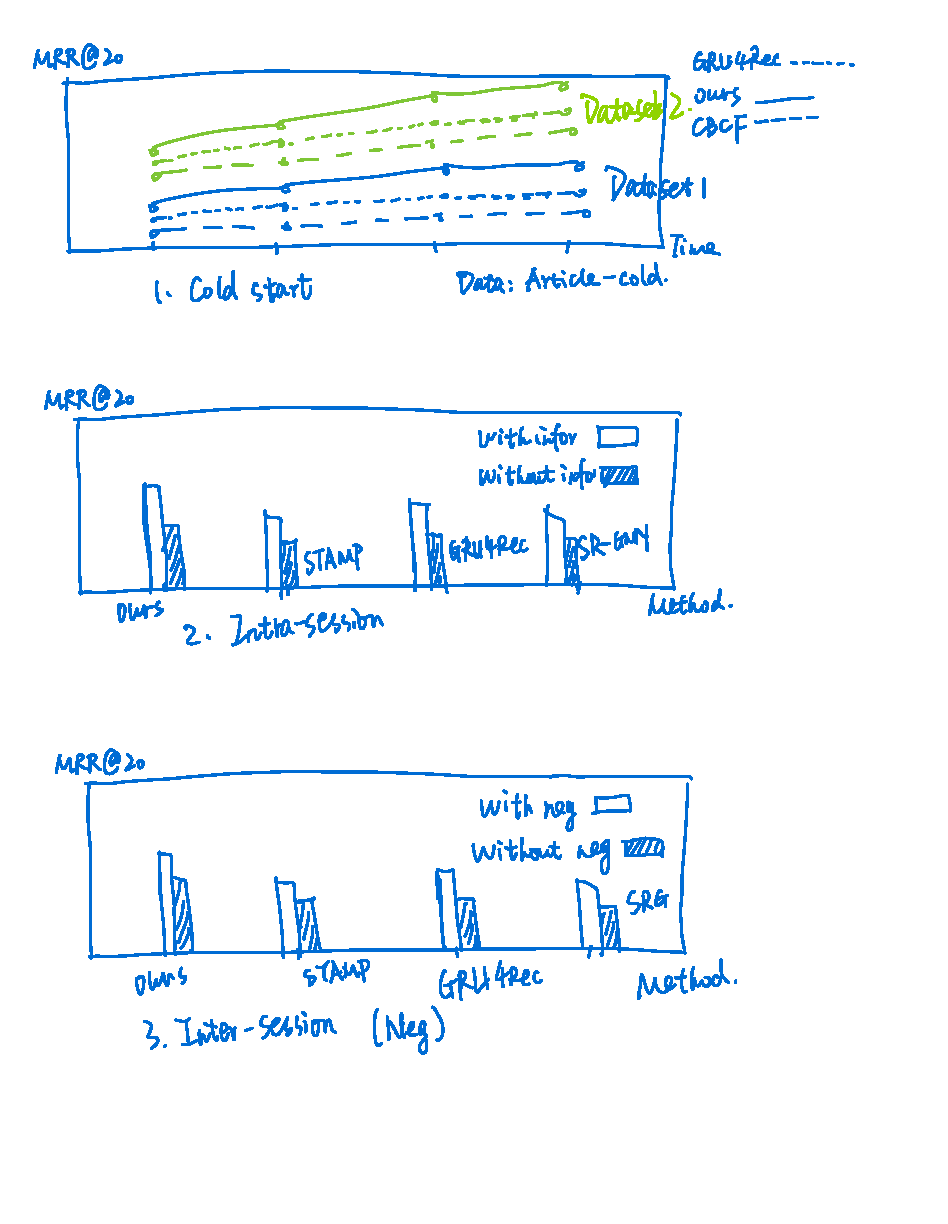
\includegraphics[width=0.9\columnwidth]{fig/ablation.pdf}
  \caption{example.}
  \label{fig:ablation}
\end{figure}
